\documentclass[10pt]{article}
\usepackage[utf8]{inputenc}
\usepackage[T1]{fontenc}
\usepackage{amsmath}
\usepackage{amsfonts}
\usepackage{amssymb}
\usepackage{mhchem}
\usepackage{stmaryrd}
\usepackage{bbold}
\usepackage{graphicx}
\usepackage[export]{adjustbox}
\graphicspath{ {./images/} }
\usepackage{mathrsfs}

\title{Chapter 25 }

\author{}
\date{}


\begin{document}
\maketitle
\section{Binary Choice}
\subsection{Introduction}
This and the next two chapters treat what are known as limited dependent variables. These are variables which have restricted support (a subset of the real line) and this restriction has consequences for econometric modeling. This chapter concerns the simplest case where $Y$ is binary, meaning that it takes two values. Without loss of generality these are taken as zero and one, thus $Y$ has support $\{0,1\}$. In econometrics we typically call this class of models binary choice.

Examples of binary dependent variables include: Purchase of a single item; Market entry; Participation; Approval of an application/patent/loan. The dependent variable may be recorded as Yes/No, True/False, or $1 /-1$, but can always be written as $1 / 0$.

The goal in binary choice analysis is estimation of the conditional or response probability $\mathbb{P}[Y=1 \mid X]$ given a set of regressors $X$. We may be interested in the response probability or some transformation such as its derivative - the marginal effect. A traditional approach to binary choice modeling (and limited dependent variable models in general) is parametric with estimation by maximum likelihood. There is also a substantial literature on semiparametric estimation. In recent years, applied practice has tilted towards linear probability models estimated by least squares.

For more detailed treatments see Maddala (1983), Cameron and Trivedi (2005), and Wooldridge (2010)

\section{$25.2$ Binary Choice Models}
Let $(Y, X)$ be random with $Y \in\{0,1\}$ and $X \in \mathbb{R}^{k}$. The response probability of $Y$ with respect to $X$ is
$$
P(x)=\mathbb{P}[Y=1 \mid X=x]=\mathbb{E}[Y \mid X=x] .
$$
The response probability completely describes the conditional distribution. The marginal effect is
$$
\frac{\partial}{\partial x} P(x)=\frac{\partial}{\partial x} \mathbb{P}[Y=1 \mid X=x]=\frac{\partial}{\partial x} \mathbb{E}[Y \mid X=x] .
$$
This equals the regression derivative. Economic applications often focus on the marginal effect.

To illustrate, consider the probability of marriage given age. We use the cps09mar dataset, take the subset of men with a college degree ( $n=6441$ ), set $Y=1$ if the individual is married or widowed but not separated or divorced ${ }^{1}$ and set $Y=0$ otherwise. The regressor is age which takes values in $[19,80]$.

${ }^{1}$ marital equals $1,2,3$, or 4. In Figure 25.1(a) we plot two estimates of $P(x)$. The filled circles are nonparametric estimates - the empirical marriage frequency for each age - and the solid line is our preferred specification (a probit spline model, described below). What seems apparant is that the probability of marriage is near zero for age $=19$, increases linearly to $80 \%$ around age $=35$, remains roughly flat at $80 \%$ for ages $40-65$, and increases for higher ages.

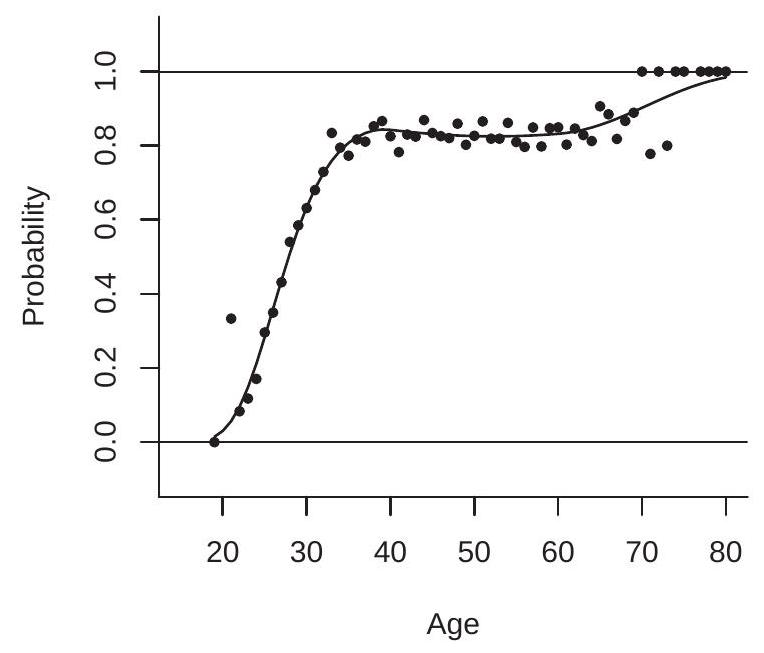
\includegraphics[max width=\textwidth]{2022_10_23_79ac6a85f9738eaa4c30g-02}

(a) Response Probabilities

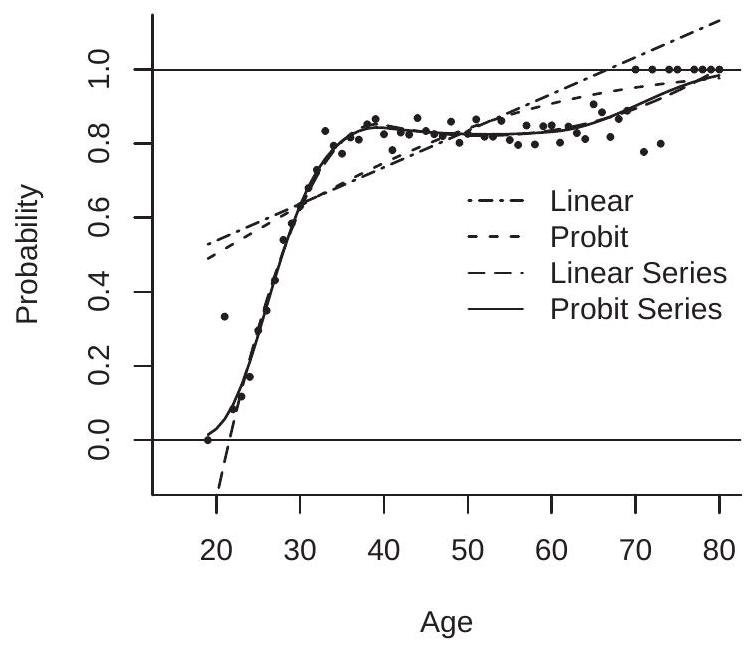
\includegraphics[max width=\textwidth]{2022_10_23_79ac6a85f9738eaa4c30g-02(1)}

(b) Binary Choice Models

Figure 25.1: Probability of Marriage Given Age for College Educated Men

The variables satisfy the regression framework
$$
\begin{aligned}
Y &=P(X)+e \\
\mathbb{E}[e \mid X] &=0 .
\end{aligned}
$$
The error $e$ is not "classical". It has the two-point conditional distribution
$$
e=\left\{\begin{array}{c}
1-P(X), \quad \text { with probability } P(X) \\
-P(X), \quad \text { with probability } 1-P(X) .
\end{array}\right.
$$
It is also highly heteroskedastic with conditional variance
$$
\operatorname{var}[e \mid X]=P(X)(1-P(X)) .
$$
Regression scatterplots with binary $Y$ are effectively useless, as the $Y$ values do not "scatter" but rather lie exclusively on the lies $y=0$ and $y-1$.

\subsection{Models for the Response Probability}
We now describe the most common models used for the response probability $P(x)$.

Linear Probability Model: $P(x)=x^{\prime} \beta$ where $\beta$ is a coefficient vector. In this model the response probability is a linear function of the regressors. The linear probability model has the advantage that it is simple to interpret. The coefficients $\beta$ equal the marginal effects (when $X$ does not include nonlinear transformations). Since the response probability equals the conditional mean this model equals the linear regression model. Linearity means that estimation is simple as least squares can be used to estimate the coefficients. In more complicated settings (e.g. panel data with fixed effects or endogenous variables with instruments) standard estimators can be employed.

A disadvantage of the linear probability model is that it does not respect the $[0,1]$ boundary. Fitted and predicted values from estimated linear probability models frequently violate these boundaries producing nonsense results.

To illustrate, in Figure 25.1(b) we plot with the dash-dotted line the linear probability model fit to the observations in the sample described in the previous section. The fitted values are a poor approximation to the response probabilities. They also violate the $[0,1]$ boundary for men above the age of 67 . According to the model an 80-year-old is married with probability $113 \%$ !

Overall, the linear probability model is a poor choice for calculation of probabilities.

Index Models: $P(x)=G\left(x^{\prime} \beta\right)$ where $G(u)$ is a link function and $\beta$ is a coefficient vector. This framework is also called a single index model where $x^{\prime} \beta$ is a linear index function. In binary choice models $G(u)$ is distribution function which respects the probability bounds $0 \leq G(u) \leq 1$. In economic applications $G(u)$ is typically the normal or logistic distribution function, both of which are symmetric about zero so that $G(-u)=1-G(u)$. We assume throughout this chapter that this symmetry condition holds. Let $g(u)=\frac{\partial}{\partial u} G(u)$ denote the density function of $G(u)$. In an index model the marginal effect function is
$$
\frac{\partial}{\partial x} P(x)=\beta g\left(x^{\prime} \beta\right) .
$$
Index models are only slightly more complicated than the linear probability model but have the advantage of respecting the $[0,1]$ boundary. The two most common index models are the probit and logit.

Probit Model: $P(x)=\Phi\left(x^{\prime} \beta\right)$ where $\Phi(u)$ is the standard normal distribution function. This is a traditional workhorse model for binary choice analysis. It is simple, easy to use, easy to interpret, and is based on the classical normal distribution.

Logit Model: $P(x)=\Lambda\left(x^{\prime} \beta\right)$ where $\Lambda(u)=(1+\exp (-u))^{-1}$ is the logistic distribution function. This is an alternative workhorse model for binary choice analysis. The logistic and normal distribution functions (appropriately scaled) have similar shapes so the probit and logit models typically produce similar estimates for the response probabilities and marginal effects. One advantage of the logit model is that the distribution function is available in closed form which speeds computation.

Linear Series Model: $P(x)=x_{K}^{\prime} \beta_{K}$ where $x_{K}=x_{K}(x)$ is a vector of transformations of $x$ and $\beta_{K}$ is a coefficient vector. A series expansion has the ability to approximate any continuous function including the response probability $P(x)$. The advantage of a linear series model is that its linear form allows the application of linear econometric methods. It is not guaranteed, however, to be boundary-respecting.

Index Series Model: $P(x)=G\left(x_{K}^{\prime} \beta_{K}\right)$ where $G(u)$ is a distribution function (either normal or logistic in practice), $x_{K}=x_{K}(x)$ is a vector of transformations of $x$, and $\beta_{K}$ is a coefficient vector. A series expansion has the ability to approximate any continuous function including the transformed response probability $G^{-1}(p(x))$. This means that the index series model has the ability to approximate any continuous response probability. In addition, the model is boundary-respecting.

To illustrate the approximating capabilities of the models view Figure 25.1(b) which plots four estimated response probability functions: (1) Linear; (2) Probit; (3) Linear Series; (4) Probit Series. The first two models are specified as linear in age. The two series models use a quadratic spline in age with kinks at 40 and 60.

As discussed earlier, in this application the linear probability model is a particularly poor fit. It overpredicts the probability for men under 30 and over 50 , under-predicts the others, and violates the $[0,1]$ boundary. The simple probit model is also quite poor. It produces an estimated response probability function which is similar to the linear probability model for ages up to 60 . Its advantage is that for ages over 60 it does not violate the $[0,1]$ boundary. In contrast, the two series models produce excellent fitted response probability functions. The two estimates are nearly identical for ages above 25 . The main difference between the estimated functions is that the probit series model provides a globally excellent fit, while the linear series model fails for ages less than 25 , severely violating the $[0,1]$ boundary. The linear series model estimates that a 19 -year-old is married with negative probability: $-27 \%$ !

To summarize, a probit series model has several excellent features. It is simple, based on a popular link function, globally approximates any continuous response probability function, and respects the $[0,1]$ boundary. A linear series model is also a reasonable candidate, but has the disadvantage of not necessarily respecting the $[0,1]$ boundary.

\section{Probit and Logit}
The intruiging labels probit and logit have a long history in statistical analysis. The term probit was coined by Chester Bliss in 1934 as a contraction of "probability unit". The logistic function was introduced by Pierre François Verhulst in 1938 as a modified exponential growth model. It is speculated that he used the term logistic as a contrast to logarithmic. In 1944 Joseph Berkson proposed a binary choice model based on the logistic distribution function. He motivated the logistic as a convenient computational approximation to the normal. As his model was an analog of the probit Berkson called his model the logit.

\subsection{Latent Variable Interpretation}
An index model can be interpreted as a latent variable model. Consider
$$
\begin{aligned}
Y^{*} &=X^{\prime} \beta+e \\
e & \sim G(e) \\
Y &=\mathbb{1}\left\{Y^{*}>0\right\}=\left\{\begin{array}{cc}
1 & \text { if } Y^{*}>0 \\
0 & \text { otherwise. }
\end{array}\right.
\end{aligned}
$$
In this model the observables are $(Y, X)$. The variable $Y^{*}$ is latent, linear in $X$ and an error $e$, with the latter drawn from a symmetric distribution $G$. The observed binary variable $Y$ equals 1 if the latent variable $Y^{*}$ exceeds zero and equals 0 otherwise.

The event $Y=1$ is the same as $Y^{*}>0$, which is the same as
$$
X^{\prime} \beta+e>0 .
$$
This means that the response probability is
$$
P(x)=\mathbb{P}\left[e>-x^{\prime} \beta\right]=1-G\left(-x^{\prime} \beta\right)=G\left(x^{\prime} \beta\right) .
$$
The final equality uses the assumption that $G(u)$ is symmetric about zero. This shows that the response probability is $P(x)=G\left(x^{\prime} \beta\right)$ which is an index model with link function $G(u)$.

This latent variable model corresponds to a choice model where $Y^{*}$ is an individual's relative utility (or profit) of the options $Y=1$ and $Y=0$, and the individual selects the option with the higher utility. We see that this structural choice model is identical to an index model with link function equalling the distribution of the error. It is a probit model if the error $e$ is standard normal and is a logit model if $e$ is logistically distributed.

You may have noticed that we have discussed cases where the error $e$ is either standard normal or standard logistic, that is, their scale is fixed. This is because the scale of the error distribution is not identified. To see this, suppose that $e=\sigma \varepsilon$ where $\varepsilon$ has a distribution $G(u)$ with unit variance. Then the response probability is
$$
\mathbb{P}[Y=1 \mid X=x]=\mathbb{P}\left[\sigma e>-x^{\prime} \beta\right]=G\left(\frac{x^{\prime} \beta}{\sigma}\right)=G\left(x^{\prime} \beta^{*}\right)
$$
where $\beta^{*}=\beta / \sigma$. This is an index model with coefficient $\beta^{*}$. This means that $\beta$ and $\sigma$ are not separately identified; only the ratio $\beta^{*}=\beta / \sigma$ is identified. The standard solution is to normalize $\sigma$ to a convenient value. The probit and logit models use the normalizations $\sigma=1$ and $\sigma=\pi / \sqrt{3} \simeq 1.8$, respectively.

Two consequences of the above analysis are that (1) interpretation of the coefficient vector $\beta$ cannot be separated from the scale of the error; and (2) the coefficients of probit and logit models cannot be compared without rescaling. In general, it is best to interpret the coefficient of a probit model as $\beta / \sigma$, the structural coefficient scaled by the stuctural standard deviation, and to interpret the coefficient of a logit model as $\beta / \nu$, the structural coefficient scaled by the structural logistic scale parameter $v=\sigma \sqrt{3} / \pi$. For a rough comparison ${ }^{2}$ of probit and logit coefficients multiply the probit coefficients by $1.8$ or divide the logit coefficients by $1.8$.

While the coefficient $\beta$ is not identified the following parameters are identified:

\begin{enumerate}
  \item Scaled coefficients: $\beta^{*}=\beta / \sigma$.

  \item Ratios of coefficients: $\beta_{1} / \beta_{2}=\beta_{1}^{*} / \beta_{2}^{*}$.

  \item Marginal effects: $\frac{\partial}{\partial x} P(x)=\frac{\beta}{\sigma} g\left(\frac{x^{\prime} \beta}{\sigma}\right)=\beta^{*} g\left(x^{\prime} \beta^{*}\right)$.

\end{enumerate}
These only depend on $\beta^{*}$ so are identified.

Concerning identification, if we take a broader nonparametric view the error distribution $G(u)$ is not identified. To see this, write the structural equation nonparametrically as $Y^{*}=m(X)+e$. The response probability is
$$
P(x)=1-G(-m(x)) .
$$
The joint distribution identifies $P(x)$. If $G(e)$ and $m(x)$ are nonparametric they cannot be separately identified from the response probability. Only the composite (25.4) is identified.

An important implication is that there is no loss of generality in setting $G(u)$ equal to a specific parametric distribution such as the normal so long as the function $m(x)$ is treated nonparametrically.

${ }^{2}$ This produces only a rough comparison as this normalization only puts the coefficients on the same scale. They are not equal since the models are different.

\subsection{Likelihood}
Probit and logit models are typically estimated by maximum likelihood. To construct the likelihood we need the distribution of an individual observation. Recall that if $Y$ is Bernoulli, such that $\mathbb{P}[Y=1]=p$ and $\mathbb{P}[Y=0]=1-p$, then $Y$ has the probability mass function
$$
\pi(y)=p^{y}(1-p)^{1-y}, \quad y=0,1 .
$$
In the index model $\mathbb{P}[Y=1 \mid X]=G\left(X^{\prime} \beta\right), Y$ is conditionally Bernoulli, so its conditional probability mass function is
$$
\pi(Y \mid X)=G\left(X^{\prime} \beta\right)^{Y}\left(1-G\left(X^{\prime} \beta\right)\right)^{1-Y}=G\left(X^{\prime} \beta\right)^{Y} G\left(-X^{\prime} \beta\right)^{1-Y}=G\left(Z^{\prime} \beta\right)
$$
where
$$
Z=\left\{\begin{array}{cc}
X & \text { if } Y=1 \\
-X & \text { if } Y=0 .
\end{array}\right.
$$
Taking logs and summing across observations we obtain the log-likelihood function:
$$
\ell_{n}(\beta)=\sum_{i=1}^{n} \log G\left(Z_{i}^{\prime} \beta\right)
$$
For the probit and logit models this is
$$
\begin{aligned}
\ell_{n}^{\text {probit }}(\beta) &=\sum_{i=1}^{n} \log \Phi\left(Z_{i}^{\prime} \beta\right) \\
\ell_{n}^{\text {logit }}(\beta) &=\sum_{i=1}^{n} \log \Lambda\left(Z_{i}^{\prime} \beta\right)
\end{aligned}
$$
Define the first and (negative) second derivatives of the log distribution function: $h(x)=\frac{d}{d x} \log G(x)$ and $H(x)=-\frac{d^{2}}{d x^{2}} \log G(x)$. For the logit model these equal (See Exercise 25.5)
$$
\begin{aligned}
&h_{\text {logit }}(x)=1-\Lambda(x) \\
&H_{\text {logit }}(x)=\Lambda(x)(1-\Lambda(x))
\end{aligned}
$$
and for the probit model (See Exercise 25.6)
$$
\begin{aligned}
h_{\text {probit }}(x) &=\frac{\phi(x)}{\Phi(x)} \stackrel{\text { def }}{=} \lambda(x) \\
H_{\text {probit }}(x) &=\lambda(x)(x+\lambda(x)) .
\end{aligned}
$$
The function $\lambda(x)=\phi(x) / \Phi(x)$ is known as the inverse Mills ratio.

Both the logit and probit have the property that $H(x)>0$. This is easily seen for the logit case because it is the product of the distribution function and its complement, but less so for the probit case. Here we make use of a convenient property of log concave ${ }^{3}$ functions: if a density $f(x)$ is log concave then the distribution function $F(x)$ is log concave. The standard normal density $\phi(x)$ is log concave ${ }^{4}$, implying that $\Phi(x)$ is log concave, implying $H_{\text {probit }}(x)>0$ as desired.

${ }^{3}$ A function $f(x)$ is $\log$ concave if $\log f(x)$ is concave.

${ }^{4} \log \phi(x)=-\log (2 \pi)-x^{2} / 2$ is concave. The likelihood score and Hessian are
$$
\begin{gathered}
S_{n}(\beta)=\frac{\partial}{\partial \beta} \ell_{n}(\beta)=\sum_{i=1}^{n} Z_{i} h\left(Z_{i}^{\prime} \beta\right) \\
\mathscr{H}_{n}(\beta)=-\frac{\partial^{2}}{\partial \beta \partial \beta^{\prime}} \ell_{n}(\beta)=\sum_{i=1}^{n} X_{i} X_{i}^{\prime} H\left(Z_{i}^{\prime} \beta\right) .
\end{gathered}
$$
Examining (25.7) we can see that $H(x)>0$ implies that $\mathscr{H}_{n}(\beta)>0$ globally in $\beta$. This in turn implies that the log-likelihood $\ell_{n}(\beta)$ is globally concave. Since both $H_{\operatorname{logit}}(x)>0$ and $H_{\text {probit }}(x)>0$ we deduce that the probit and logit log likelihood functions $\ell_{n}^{\text {probit }}(\beta)$ and $\ell_{n}^{\operatorname{logit}}(\beta)$ are globally concave in $\beta$.

The MLE is the value which maximizes $\ell_{n}(\beta)$. We write this as
$$
\begin{aligned}
\widehat{\beta}^{\text {probit }} &=\underset{\beta}{\operatorname{argmax}} \ell_{n}^{\text {probit }}(\beta) \\
\widehat{\beta}^{\text {logit }} &=\underset{\beta}{\operatorname{argmax}} \ell_{n}^{\text {logit }}(\beta) .
\end{aligned}
$$
Since the probit and logit log-likelihoods are globally concave $\widehat{\beta}^{\text {probit }}$ and $\widehat{\beta}^{\text {logit }}$ are unique. There is no explicit solution so they need to be found numerically. As the log likelihoods are smooth, concave, with known first and second derivatives, numerical optimization is straightforward.

In Stata, use the commands probit and logit to obtain the MLE. In R, use the commands
$$
\begin{aligned}
&\operatorname{glm}\left(Y^{\sim} X, f a m i l y=b i n o m i a l(\text { ink="probit")) }\right. \\
&\operatorname{glm}\left(Y^{\sim} X,\right. \text { family=binomial (link="logit")). }
\end{aligned}
$$

\subsection{Pseudo-True Values}
The expected log mass function is
$$
\ell(\beta)=\mathbb{E}\left[\log G\left(Z^{\prime} \beta\right)\right] .
$$
The model is correctly specified if there is a coefficient $\beta_{0}$ such that $\mathbb{P}[Y=1 \mid X]=G\left(X^{\prime} \beta_{0}\right)$. When this holds then $\beta_{0}$ has the property that it maximizes $\ell(\beta)$ and thus satisfies
$$
\beta_{0}=\underset{\beta}{\operatorname{argmax}} \ell(\beta) .
$$
We say that the model is misspecified if there is no $\beta$ such that $\mathbb{P}[Y=1 \mid X]=G\left(X^{\prime} \beta\right)$. In this case we view the model $G\left(X^{\prime} \beta\right)$ as an approximation to the response probability and define the pseudo-true coefficient $\beta_{0}$ as the value which satisfies (25.8). By construction, (25.8) equals the true coefficient when the model is correctly specified and otherwise produces the best-fitting model with respect to the expected $\log$ mass function.

When the distribution function $G(x)$ is log concave (as it is for the probit and logit models) then $\ell(\beta)$ is globally concave. To see this define
$$
\boldsymbol{Q}(\beta)=-\frac{\partial^{2}}{\partial \beta \partial \beta^{\prime}} \ell(\beta)=\mathbb{E}\left[X X^{\prime} H\left(Z^{\prime} \beta\right)\right]
$$
and observe that $H(x)>0$ (by log concavity), which implies $\boldsymbol{Q}(\beta) \geq 0$, which implies that $\ell(\beta)$ is globally concave. Furthermore, the minimizer (25.8) is unique under the full rank condition
$$
\mathbb{E}\left[X X^{\prime} H\left(X^{\prime} \beta_{0}\right)\right]>0 .
$$
It is important to note that the concavity of $\ell(\beta)$ and uniqueness of the maximizer $\beta_{0}$ are properties of the model $G\left(X^{\prime} \beta\right)$ not the true distribution.

For specificity, for the probit and logit models define the population criterions
$$
\begin{aligned}
\ell^{\operatorname{probit}^{\prime}(\beta)} &=\mathbb{E}\left[\log \Phi\left(Z^{\prime} \beta\right)\right] \\
\ell^{\operatorname{logit}}(\beta) &=\mathbb{E}\left[\log \Lambda\left(Z^{\prime} \beta\right)\right]
\end{aligned}
$$
and the pseudo-true values
$$
\begin{aligned}
\beta^{\text {probit }} &=\underset{\beta}{\operatorname{argmax}} \ell^{\text {probit }}(\beta) \\
\beta^{\text {logit }} &=\underset{\beta}{\operatorname{argmax}} \ell^{\text {logit }}(\beta) .
\end{aligned}
$$
We now describe the full rank condition (25.9) for the logit and probit models. For the probit model $H_{\text {logit }}(-x)=H_{\text {logit }}(x)$ is symmetric about zero, so $H_{\text {logit }}\left(Z^{\prime} \beta\right)=H_{\text {logit }}\left(X^{\prime} \beta\right)=\Lambda\left(X^{\prime} \beta\right)\left(1-\Lambda\left(X^{\prime} \beta\right)\right)$. We deduce that $(25.9)$ is the same as
$$
\boldsymbol{Q}_{\text {logit }} \stackrel{\text { def }}{=} \mathbb{E}\left[X X^{\prime} \Lambda\left(X^{\prime} \beta^{\text {logit }}\right)\left(1-\Lambda\left(X^{\prime} \beta^{\text {logit }}\right)\right)\right]>0 .
$$
For the probit model the condition (25.9) is
$$
\boldsymbol{Q}_{\text {probit }} \stackrel{\text { def }}{=} \mathbb{E}\left[X X^{\prime} H_{\text {probit }}\left(Z^{\prime} \beta^{\text {probit }}\right)\right]>0 .
$$
When (25.10) and/or (25.11) hold the population minimizers $\beta^{\text {probit }}$ and/or $\beta^{\text {logit }}$ are unique.

\subsection{Asymptotic Distribution}
We first provide conditions for consistent estimation. Let $B$ be the parameter space for $\beta$.

Theorem 25.1 Consistency of Logit Estimation. If (1) $\left(Y_{i}, X_{i}\right)$ are i.i.d.; (2) $\mathbb{E}\|X\|<\infty$; (3) $\boldsymbol{Q}_{\text {logit }}>0$; and (4) B is compact; then $\widehat{\beta}^{\operatorname{logit}} \underset{p}{\longrightarrow} \beta^{\operatorname{logit}}$ as $n \rightarrow \infty$.

Theorem 25.2 Consistency of Probit Estimation. If (1) $\left(Y_{i}, X_{i}\right)$ are i.i.d.; (2) $\mathbb{E}\|X\|^{2}<\infty$; (3) $\boldsymbol{Q}_{\text {probit }}>0$; and (4) B is compact; then $\widehat{\beta}^{\text {probit }} \underset{p}{\longrightarrow} \beta^{\text {probit }}$ as $n \rightarrow \infty$

The proofs are in Section 25.14. To derive the asymptotic distributions we appeal to Theorem $22.4$ for m-estimators which shows that the asymptotic distribution is normal with a covariance matrix $V=$ $\boldsymbol{Q}^{-1} \Omega \boldsymbol{Q}^{-1}$ where $\boldsymbol{Q}$ is defined in (25.10) for the logit model and is defined in (25.11) for the probit model. The variance of the score is $\Omega=\mathbb{E}\left[X X^{\prime} h\left(Z^{\prime} \beta\right)^{2}\right]$. In the logit model we have the simplification
$$
\Omega_{\text {logit }}=\mathbb{E}\left[X X^{\prime}\left(Y-\Lambda\left(X^{\prime} \beta^{\text {logit }}\right)\right)^{2}\right]
$$
(explained below). We do not have a similar simplification for the probit model (except under correct specification, discussed below) and thus define
$$
\Omega_{\text {probit }}=\mathbb{E}\left[X X^{\prime} \lambda\left(Z^{\prime} \beta^{\text {probit }}\right)^{2}\right] .
$$
To see (25.12), with some algebra you can show that
$$
h\left(Z^{\prime} \beta\right)^{2}=\frac{g\left(X^{\prime} \beta\right)^{2}}{G\left(X^{\prime} \beta\right)^{2}} Y+\frac{g\left(X^{\prime} \beta\right)^{2}}{\left(1-G\left(X^{\prime} \beta\right)\right)^{2}}(1-Y)=\frac{g\left(X^{\prime} \beta\right)^{2}\left(Y-G\left(X^{\prime} \beta\right)\right)^{2}}{G\left(X^{\prime} \beta\right)^{2}\left(1-G\left(X^{\prime} \beta\right)\right)^{2}} .
$$
In the logit model the right side simplifies to $\left(Y-\Lambda\left(X^{\prime} \beta\right)\right)^{2}$. This implies
$$
\Omega_{\text {logit }}=\mathbb{E}\left[X X^{\prime} h_{\text {logit }}\left(Z^{\prime} \beta\right)^{2}\right]=\mathbb{E}\left[X X^{\prime}\left(Y-\Lambda\left(X^{\prime} \beta^{\text {logit }}\right)\right)^{2}\right]
$$
as claimed.

Theorem 25.3 If the conditions of Theorem $25.1$ hold plus $\mathbb{E}\|X\|^{4}<\infty$ and $\beta^{\text {logit }}$ is in the interior of $B$; then as $n \rightarrow \infty$
$$
\sqrt{n}\left(\widehat{\beta}^{\text {logit }}-\beta^{\text {logit }}\right) \underset{d}{\longrightarrow} \mathrm{N}\left(0, \boldsymbol{V}_{\text {logit }}\right)
$$
where $V_{\text {logit }}=Q_{\text {logit }}^{-1} \Omega_{\text {logit }} Q_{\text {logit }}^{-1}$

Theorem 25.4 If the conditions of Theorem $25.2$ hold plus $\mathbb{E}\|X\|^{4}<\infty$ and $\beta^{\text {probit }}$ is in the interior of $B$; then as $n \rightarrow \infty$
$$
\sqrt{n}\left(\widehat{\beta}^{\text {probit }}-\beta^{\text {probit }}\right) \underset{d}{\longrightarrow} \mathrm{N}\left(0, \boldsymbol{V}_{\text {probit }}\right)
$$
where $\boldsymbol{V}_{\text {probit }}=\boldsymbol{Q}_{\text {probit }}^{-1} \Omega_{\text {probit }} \boldsymbol{Q}_{\text {probit }}^{-1}$

The proofs are in Section $25.14$.

Under correct specification the information matrix equality implies the simplifications $\boldsymbol{V}_{\text {logit }}=\boldsymbol{Q}_{\operatorname{logit}}^{-1}$ and $\boldsymbol{V}_{\text {probit }}=\boldsymbol{Q}_{\text {probit }}^{-1}$. We also have the simplification
$$
\Omega_{\text {probit }}=\boldsymbol{Q}_{\text {probit }}=\mathbb{E}\left[X X^{\prime} \lambda\left(X^{\prime} \beta^{\text {probit }}\right) \lambda\left(-X^{\prime} \beta^{\text {probit }}\right)\right] .
$$
This follows from (25.14), which for the probit model can be written as
$$
\lambda\left(Z^{\prime} \beta\right)^{2}=\lambda\left(X^{\prime} \beta\right) \lambda\left(-X^{\prime} \beta\right) \frac{\left(Y-\Phi\left(X^{\prime} \beta\right)\right)^{2}}{\Phi\left(X^{\prime} \beta\right)\left(1-\Phi\left(X^{\prime} \beta\right)\right)} .
$$
Under correct specification $\mathbb{E}[Y \mid X]=\Phi\left(X^{\prime} \beta\right)$ and $\mathbb{E}\left[\left(Y-\Phi\left(X^{\prime} \beta\right)\right)^{2} \mid X\right]=\Phi\left(X^{\prime} \beta\right)\left(1-\Phi\left(X^{\prime} \beta\right)\right)$. Taking expectations given $X$ the above expression simplifies to $\lambda\left(X^{\prime} \beta\right) \lambda\left(-X^{\prime} \beta\right)$. Inserted into (25.13) yields (25.15).

\section{$25.8$ Covariance Matrix Estimation}
For the logit model define $\widehat{\Lambda}_{i}=\Lambda\left(X_{i}^{\prime} \widehat{\beta}^{\text {logit }}\right)$ and
$$
\begin{aligned}
&\widehat{\boldsymbol{Q}}_{\text {logit }}=\frac{1}{n} \sum_{i=1}^{n} X_{i} X_{i}^{\prime} \widehat{\Lambda}_{i}\left(1-\widehat{\Lambda}_{i}\right) \\
&\widehat{\Omega}_{\text {logit }}=\frac{1}{n} \sum_{i=1}^{n} X_{i} X_{i}^{\prime}\left(Y_{i}-\widehat{\Lambda}_{i}\right)^{2}
\end{aligned}
$$
The sandwich covariance matrix estimator for $\boldsymbol{V}_{\text {logit }}$ is $\widehat{\boldsymbol{V}}_{\text {logit }}=\widehat{\boldsymbol{Q}}_{\text {logit }}^{-1} \widehat{\Omega}_{\text {logit }} \widehat{\boldsymbol{Q}}_{\text {logit }}^{-1}$. Under the assumption of correct specification we may alternatively use $\widehat{\boldsymbol{V}}_{\text {logit }}^{0}=\widehat{\boldsymbol{Q}}_{\operatorname{logit}}^{-1}$.

For the probit model define $\widehat{\mu}_{i}=Z_{i}^{\prime} \widehat{\beta}^{\text {probit }}, \widehat{\lambda}_{i}=\lambda\left(\widehat{\mu}_{i}\right)$, and
$$
\begin{aligned}
&\widehat{\boldsymbol{Q}}_{\text {probit }}=\frac{1}{n} \sum_{i=1}^{n} X_{i} X_{i}^{\prime} \widehat{\lambda}_{i}\left(\widehat{\mu}_{i}+\widehat{\lambda}_{i}\right) \\
&\widehat{\Omega}_{\text {probit }}=\frac{1}{n} \sum_{i=1}^{n} X_{i} X_{i}^{\prime} \widehat{\lambda}_{i}^{2} .
\end{aligned}
$$
The sandwich covariance matrix estimator for $\boldsymbol{V}_{\text {probit }}$ is $\widehat{\boldsymbol{V}}_{\text {probit }}=\widehat{\boldsymbol{Q}}_{\text {probit }}^{-1} \widehat{\Omega}_{\text {probit }} \widehat{\boldsymbol{Q}}_{\text {probit }}^{-1}$ Under the assumption of correct specification we may alternatively use
$$
\widehat{\boldsymbol{Q}}_{\mathrm{probit}}^{0}=\frac{1}{n} \sum_{i=1}^{n} X_{i} X_{i}^{\prime} \lambda\left(X^{\prime} \widehat{\beta}^{\text {probit }}\right) \lambda\left(-X^{\prime} \widehat{\beta}^{\text {probit }}\right)
$$
and $\widehat{\boldsymbol{V}}_{\text {probit }}^{0}=\left(\widehat{\boldsymbol{Q}}^{0}\right)^{-1}$.

In Stata and R the default covariance matrix and standard errors are calculated by $\widehat{\boldsymbol{V}}_{\text {logit }}^{0}$ and $\widehat{\boldsymbol{V}}_{\text {probit }}^{0}$. For the robust covariance matrix estimation and standard errors $\widehat{\boldsymbol{V}}_{\text {logit }}$ and $\widehat{\boldsymbol{V}}_{\text {probit }}$, in Stata use the option vce(robust). In R use the package sandwich which has options for the HC0, HC1, and HC2 (and other) covariance matrix estimators.

\subsection{Marginal Effects}
As we mentioned before it is common to focus on marginal effects rather than coefficients as the latter are difficult to interpret. In this section we describe marginal effects in more detail and describe common estimators.

Take the index model $\mathbb{P}[Y=1 \mid X=x]=G\left(x^{\prime} \beta\right)$ when $x$ does not include nonlinear transformations. In this case the marginal effects are
$$
\delta(x)=\frac{\partial}{\partial x} P(x)=\beta g\left(x^{\prime} \beta\right) .
$$
This varies with $x$. For example, in Figure $25.1$ we see that the marginal effect of age on marriage probability is about $0.06$ per year for ages between 20 and 30, but is close to zero for ages above 40 .

For reporting it is typical to calculate an "average" value. There are more than one way to do so. The most common is the average marginal effect
$$
\mathrm{AME}=\mathbb{E}[\delta(X)]=\beta \mathbb{E}\left[g\left(X^{\prime} \beta\right)\right] .
$$
An estimator of $\delta(x)$ is $\widehat{\delta}(x)=\widehat{\beta} g\left(x^{\prime} \widehat{\beta}\right)$. An estimator of the AME is
$$
\widehat{\mathrm{AME}}=\frac{1}{n} \sum_{i=1}^{n} \widehat{\delta}\left(X_{i}\right)=\widehat{\beta} \frac{1}{n} \sum_{i=1}^{n} g\left(X_{i}^{\prime} \widehat{\beta}\right) .
$$
When the vector $X$ includes nonlinear transformations the marginal effects need to be carefully defined. For example, in the model $\mathbb{P}[Y=1 \mid X=x]=G\left(\beta_{0}+\beta_{1} x+\cdots+\beta_{p} x^{p}\right)$ the marginal effect is
$$
\delta(x)=\left(\beta_{1}+\cdots+p \beta_{p} x^{p-1}\right) g\left(\beta_{0}+\beta_{1} x+\cdots+\beta_{p} x^{p}\right) .
$$
An estimator of $\delta(x)$ is
$$
\widehat{\delta}(x)=\left(\widehat{\beta}_{1}+\cdots+p \widehat{\beta}_{p} x^{p-1}\right) g\left(\widehat{\beta}_{0}+\widehat{\beta}_{1} x+\cdots+\widehat{\beta}_{p} x^{p}\right) .
$$
An estimator of the AME is $\widehat{\mathrm{AME}}=\frac{1}{n} \sum_{i=1}^{n} \widehat{\delta}\left(X_{i}\right)$

In Stata, marginal effects can be estimated with margins , $\mathrm{dydx}(*)$.

\subsection{Application}
We illustrate with an application to the probability of marriage using the cps09mar dataset. We use the subsample of men with ages up to 35 ( $n=9137)$. We include as regressors an individual's age, education, and indicators for Black, Asian, Hispanic, and three regions. We estimate linear logit and linear probit models, calculate coefficients and average marginal effects, and report robust standard errors. The results are reported in Table $25.1$.

Reading the tables you will see that the logit and probit coefficient estimates all have the same signs but the logit coefficients are larger in magnitude. We see that the probability of marriage is increasing in age, is lower for Black individuals, and varies across geographic regions. The coefficients themselves are difficult to intepret so it is better to focus on the estimated marginal effects. Doing so, we see that the logit and probit estimates are essentially identical. This is a common finding in empirical applications when both provide good approximations to the response probability. Examining the coefficients further we see that the probability of marriage increases about $4.5 \%$ for each year of age. The point estimate of the impact of education is $0.3 \%$ per year of education, which is a small magnitude. Black men are married with a reduced probability of $15 \%$ relative to the omitted category (men who are not Black, Asian, nor Hispanic). The estimated marginal effects for Asian and Hispanic men are small ( $1 \%$ and $-2 \%$, respectively) relative to the omitted category. Comparing regions we see that marriage rates are about 6 8\% higher in the Midwest, South, and West relative to the NorthEast (the omitted category). Equivalently, men in the NorthEast have a reduced probability of about $7 \%$ relative to the rest of the country.

Two messages from this application are that the choice of logit versus probit is unimportant and that it is better to focus on marginal effects than coefficients. A hidden message is that (as for all econometric applications) model specification is critically important. The estimates in Table $25.1$ are for men with ages 19-35. This choice was made so that the response probability would be well modeled with a single linear term in age. If instead the estimates were calculated on the full sample (and still using a linear specification) then the estimated marginal effect of age would have been $1 \%$ per year rather than $4.5 \%$, a large mis-estimate of the effect of age on marriage probability.

\subsection{Semiparametric Binary Choice}
The semiparametric binary choice model is
$$
\mathbb{P}[Y=1 \mid X]=G\left(X^{\prime} \beta\right)
$$
Table 25.1: Binary Choice Regressions for Marriage

\begin{tabular}{lcccc}
\hline\hline
 & \multicolumn{2}{c}{Logit} & \multicolumn{2}{c}{Probit} \\
 & Coefficient & AME & Coefficient & AME \\
\cline { 2 - 5 }
age & $0.217$ & $0.044$ & $0.132$ & $0.045$ \\
 & $(0.006)$ & $(0.001)$ & $(0.003)$ & $(0.001)$ \\
education & $0.014$ & $0.003$ & $0.009$ & $0.003$ \\
 & $(0.010)$ & $(0.002)$ & $(0.006)$ & $(0.002)$ \\
Black & $-0.767$ & $-0.156$ & $-0.454$ & $-0.153$ \\
 & $(0.092)$ & $(0.018)$ & $(0.054)$ & $(0.018)$ \\
Asian & $0.033$ & $0.007$ & $0.025$ & $0.008$ \\
 & $(0.103)$ & $(0.021)$ & $(0.063)$ & $(0.021)$ \\
Hispanic & $-0.084$ & $-0.017$ & $-0.048$ & $-0.017$ \\
 & $(0.063)$ & $(0.013)$ & $(0.038)$ & $(0.013)$ \\
MidWest & $0.272$ & $0.056$ & $0.165$ & $0.056$ \\
 & $(0.074)$ & $(0.011)$ & $(0.045)$ & $(0.015)$ \\
South & $0.338$ & $0.069$ & $0.203$ & $0.069$ \\
 & $(0.070)$ & $(0.014)$ & $(0.043)$ & $(0.014)$ \\
West & $0.383$ & $0.078$ & $0.228$ & $0.077$ \\
 & $(0.072)$ & $(0.015)$ & $(0.044)$ & $(0.015)$ \\
Intercept & $-6.45$ &  & $-3.93$ &  \\
 & $(0.21)$ &  & $(0.12)$ &  \\
\hline
\end{tabular}

where $G(x)$ is unknown. Interest typically focuses on the coefficients $\beta$.

In the latent variable framework $G(x)$ is the distribution function of a latent error $e$. As it is not credible that the distribution $G(x)$ is known, the semiparametric model treats $G(x)$ as unknown. The goal is to estimate the coefficient $\beta$ while agnostic about $G(x)$.

There are many contributions to this literature. Two of the most influential are Manski (1975) and Klein and Spady (1993). Both use the latent variable framework $Y^{*}=X^{\prime} \beta+e$.

Manksi (1975) shows that $\beta$ is identified up to scale if med $[e \mid X]=0$. He proposes a clever maximum score estimator is which is consistent for $\beta$ up to scale under this weak condition. His method, however, does not permit estimation of the response probabilities nor marginal effects because his assumptions are insufficient to identify $G(x)$.

Klein and Spady (1993) add the assumption that $e$ is independent of $X$ which implies identification of $G(x)$. They propose simultaneous estimation of $\beta$ and $G(x)$ based on the following two properties: (1) If $G(x)$ is known then $\beta$ can be estimated by maximum likelihood; (2) If $\beta$ is known then $G(x)$ can be estimated by nonparametric regression of $Y$ on $X^{\prime} \beta$. Combining these two properties into a nested criterion, they produce a consistent, asymptotically normal, and efficient estimator of $\beta$.

While the ideas of Manski and Klein-Spady are quite clever, the trouble is that model $G\left(x^{\prime} \beta\right)$ relies on the parametric linear index assumption. Suppose we relax the latter to a nonparametric function $m(x)$ but assume that $e$ is independent of $X$. Then the response probability is $1-G(-m(x))$. In this case neither $G(x)$ nor $m(x)$ is identifed; only the composite function $G(-m(x))$ is identified. This means that estimation of $m(x)$ while agnostic about $G(x)$ is impossible without a parametric assumption on $m(x)$. Consequently, the modern view is to take $P(x)=\mathbb{P}[Y=1 \mid X=x]$ as nonparametrically identified. Consistent estimation can be achieved through a series approximation, either using a linear, probit, or logit link. From this viewpoint there is no gain from the restriction to the function form $G\left(x^{\prime} \beta\right)$, and hence no gain from the semiparametric approach.

\subsection{Probit}
A latent variable structural equation model is
$$
\begin{aligned}
Y_{1}^{*} &=X^{\prime} \beta_{1}+Y_{2} \beta_{2}+e_{1} \\
Y_{2} &=X^{\prime} \gamma_{1}+Z^{\prime} \gamma_{2}+e_{2} \\
Y_{1} &=\mathbb{1}\left\{Y_{1}^{*}>0\right\} .
\end{aligned}
$$
In this model, $Y_{2}$ is scalar, endogenous, and continuously distributed, $X$ are included exogenous regressors, and $Z$ are excluded exogenous instruments.

The standard estimation method is maximum likelihood based on the assumption that the errors are jointly normal
$$
\left(\begin{array}{l}
e_{1} \\
e_{2}
\end{array}\right) \mid(X, Z) \sim \mathrm{N}\left(\left(\begin{array}{l}
0 \\
0
\end{array}\right),\left(\begin{array}{cc}
1 & \sigma_{12} \\
\sigma_{21} & \sigma_{2}^{2}
\end{array}\right)\right) .
$$
The likelihood is derived as follows. The regression of $e_{1}$ on $e_{2}$ equals
$$
\begin{aligned}
e_{1} &=\rho e_{2}+\varepsilon \\
\rho &=\frac{\sigma_{12}}{\sigma_{2}^{2}} \\
\varepsilon & \sim \mathrm{N}\left(0, \sigma_{\varepsilon}^{2}\right) \\
\sigma_{\varepsilon}^{2} &=1-\frac{\sigma_{12}^{2}}{\sigma_{2}^{2}} .
\end{aligned}
$$
Using these relationships we can write the structural equation as
$$
\begin{aligned}
Y_{1}^{*} &=\mu(\theta)+\varepsilon \\
\mu(\theta) &=X^{\prime} \beta_{1}+Y_{2} \beta_{2}+\rho\left(Y_{2}-X^{\prime} \gamma_{1}-Z^{\prime} \gamma_{2}\right) .
\end{aligned}
$$
The error $\varepsilon$ is independent of $e_{2}$ and hence of $Y_{2}$. Thus the conditional distribution of $Y_{1}^{*}$ is $\mathrm{N}\left(\mu(\theta), \sigma_{\varepsilon}^{2}\right)$. It follows that the joint density for $\left(Y_{1}, Y_{2}\right)$ is
$$
\Phi\left(\frac{\mu(\theta)}{\sigma_{\varepsilon}}\right)^{Y_{1}}\left(1-\Phi\left(\frac{\mu(\theta)}{\sigma_{\varepsilon}}\right)\right)^{1-Y_{1}} \frac{1}{\sigma_{2}} \phi\left(\frac{Y_{2}-X^{\prime} \gamma_{1}-Z^{\prime} \gamma_{2}}{\sigma_{2}}\right) .
$$
The parameter vector is $\theta=\left(\beta_{1}, \beta_{2}, \gamma_{1}, \gamma_{2}, \rho, \sigma_{\varepsilon}^{2}, \sigma_{2}^{2}\right)$.

The joint log-likelihood for a random sample $\left\{Y_{1 i}, Y_{2 i}, X_{i}, Z_{i}\right\}$ is
$$
\begin{aligned}
\ell_{n}(\theta) &=\sum_{i=1}^{n}\left[Y_{1 i} \log \Phi\left(\frac{\mu_{i}(\theta)}{\sigma_{\varepsilon}}\right)+\left(1-Y_{1 i}\right) \log \left(1-\Phi\left(\frac{\mu_{i}(\theta)}{\sigma_{\varepsilon}}\right)\right)\right] \\
&-\frac{n}{2} \log (2 \pi)-\frac{n}{2} \log \sigma_{2}^{2}-\frac{1}{2 \sigma_{2}^{2}} \sum_{i=1}^{n}\left(Y_{2 i}-X_{i}^{\prime} \gamma_{1}-Z_{i}^{\prime} \gamma_{2}\right)^{2}
\end{aligned}
$$
The maximum likelihood estimator $\widehat{\theta}$ is found by numerically maximizing $\ell_{n}(\theta)$.

The probit assumption (the treatment of $\left(e_{1}, e_{2}\right)$ as jointly normal) is important for this derivation as it allows a simple factorization of the joint distribution into the conditional distribution of $Y_{1}$ given $Y_{2}$ and the marginal distribution of $Y_{2}$. A similar factorization is not easily accomplished in a logit framework.

In Stata this estimator can be implemented with the ivprobit command.

\subsection{Binary Panel Data}
A binary choice panel model is typically written as
$$
\begin{aligned}
&Y_{i t}^{*}=X_{i t}^{\prime} \beta+u_{i}+e_{i t} \\
&Y_{i t}=\mathbb{1}\left\{Y_{i t}^{*}>0\right\} .
\end{aligned}
$$
Here, the observations are $\left(Y_{i t}, X_{i t}\right)$ for $i=1, \ldots, n$ and $t=1, \ldots, T$ with $Y_{i t}$ binary. For example, $Y_{i t}$ could denote the decision of individual $i$ to make a purchase in period $t$. The individual effect $u_{i}$ is intended to capture the feature that some individuals $i$ make purchases more (or less) frequently than can be explained by the regressors.

As in linear models there is a distinction between treating the individual effect $u_{i}$ as random (meaning that it is independent of the regressors) or fixed (meaning that it is correlated with the regressors).

Under the random effects assumption the model can be estimated by maximum likelihood. This is called random effects probit or random effects logit depending on the error distribution.

Allowing for fixed effects is more complicated. The individual effect cannot be eliminated by a linear operation because $Y_{i t}$ is a nonlinear function of $u_{i}$. For example, the transformation
$$
\Delta Y_{i t}=\mathbb{1}\left\{Y_{i t}^{*}>0\right\}-\mathbb{1}\left\{Y_{i, t-1}^{*}>0\right\}
$$
does not eliminate $u_{i}$.

Consequently there is no fixed effects estimator for the probit model. However, for the logit model Chamberlain $(1980,1984)$ developed a fixed effects estimator based on a conditional likelihood. He showed that a feature of the logistic distribution is that the individual effect can be eliminated via odds ratios, allowing the calculation of the likelihood conditional on the sum of the dependent variable.

We illustrate the construction of the likelihood for the case $T=2$. Let $Y_{i 1}, Y_{i 2}$ denote the outcomes and $N_{i}=Y_{i 1}+Y_{i 2}$ denote their sum. We calculate the conditional distribution of $\left(Y_{i 1}, Y_{i 2}\right)$ given $N_{i}$. This is the distribution of the choices given the total number of choices.

When $N_{i}=0$ or $N_{i}=2$ the likelihood is trivial. That is,
$$
\begin{aligned}
&\mathbb{P}\left[Y_{i t}=0 \mid N_{i}=0\right]=0 \\
&\mathbb{P}\left[Y_{i t}=1 \mid N_{i}=2\right]=1 .
\end{aligned}
$$
This does not depend on $\beta$, so does not affect estimation. Thus we focus exclusively on the case $N_{i}=1$.

The choice probabilities are
$$
\begin{aligned}
&\mathbb{P}\left[Y_{i t}=0\right]=\frac{\exp \left(-X_{i t}^{\prime} \beta-u_{i}\right)}{1+\exp \left(-X_{i t}^{\prime} \beta-u_{i}\right)} \\
&\mathbb{P}\left[Y_{i t}=1\right]=\frac{1}{1+\exp \left(-X_{i t}^{\prime} \beta-u_{i}\right)} .
\end{aligned}
$$
Their ratio is
$$
\frac{\mathbb{P}\left[Y_{i t}=0\right]}{\mathbb{P}\left[Y_{i t}=1\right]}=\exp \left(-X_{i t}^{\prime} \beta-u_{i}\right) .
$$
Taking a further ratio for $t=1$ and $t=2$ we obtain
$$
\frac{\mathbb{P}\left[Y_{i 1}=0\right]}{\mathbb{P}\left[Y_{i 1}=1\right]} \frac{\mathbb{P}\left[Y_{i 2}=1\right]}{\mathbb{P}\left[Y_{i 2}=0\right]}=\frac{\exp \left(-X_{1 t}^{\prime} \beta-u_{i}\right)}{\exp \left(-X_{2 t}^{\prime} \beta-u_{i}\right)}=\exp \left(\left(X_{2 t}-X_{1 t}\right)^{\prime} \beta\right) .
$$
This does not depend on the fixed effect $u_{i}$. It is a function only of the change in the regressors $\Delta X_{i}=$ $X_{i 2}-X_{i 1}$

This is effectively a nonlinear within transformation. This odds ratio eliminates dependence on the individual effect due to the exponential structure of the logistic distribution. This is special to the logit model and allows construction of a conditional likelihood function which is free of $u_{i}$.

Consider the choice probability for period 1 given $N_{i}=1$. It is
$$
\begin{aligned}
\mathbb{P}\left[Y_{i 1}=1 \mid N_{i}=1\right] &=\frac{\mathbb{P}\left[Y_{i 1}=1, Y_{i 2}=0\right]}{\mathbb{P}\left[Y_{i 1}=1, Y_{i 2}=0\right]+\mathbb{P}\left[Y_{i 1}=0, Y_{i 2}=1\right]} \\
&=\frac{\mathbb{P}\left[Y_{i 1}=1\right] \mathbb{P}\left[Y_{i 2}=0\right]}{\mathbb{P}\left[Y_{i 1}=1\right] \mathbb{P}\left[Y_{i 2}=0\right]+\mathbb{P}\left[Y_{i 1}=0\right] \mathbb{P}\left[Y_{i 2}=1\right]} \\
&=\frac{1}{1+\frac{\mathbb{P}\left[Y_{i 1}=0\right]}{\mathbb{P}\left[Y_{i 1}=1\right]} \frac{\mathbb{P}\left[Y_{i 2}=1\right]}{\mathbb{P}\left[Y_{i 2}=0\right]}} \\
&=\frac{1}{1+\exp \left(\Delta X_{i}^{\prime} \beta\right)} \\
&=1-\Lambda\left(\Delta X_{i}^{\prime} \beta\right) .
\end{aligned}
$$
Similarly $\mathbb{P}\left[Y_{i 1}=0 \mid N_{i}=1\right]=\Lambda\left(\Delta X_{i}^{\prime} \beta\right)$. Together the log-likelihood function is
$$
\ell_{n}(\beta)=\sum_{i=1}^{n} \mathbb{1}\left\{N_{i}=1\right\}\left[\left(1-Y_{i 1}\right) Y_{2 i} \log \Lambda\left(\Delta X_{i}^{\prime} \beta\right)+Y_{i 1}\left(1-Y_{i 2}\right) \log \left(1-\Lambda\left(\Delta X_{i t}^{\prime} \beta\right)\right)\right] .
$$
This conditional likelihood is free of the individual effect. Since the conditional likelhood can be computed it can be maximized to obtain the conditional likelihood estimator.

In order for the likelihood to be a non-degenerate function of $\beta$ it is necessary for there to be individuals who are switchers (select $Y=0$ in one period and $Y=1$ in the other period) and that switchers have time-varying regressors. Coefficients for time-invariant regressors are not identified.

Our derivation focused on $T=2$. The extension to $T>2$ is similar but is algebraically complicated.

In Stata, random effects probit is implemented with xtoprobit and random effects logit with xtologit. Fixed effects probit can be implemented with xtologit, fe or clogit.

\subsection{Technical Proofs*}
Proof of Theorem 25.1: The MLE $\widehat{\beta}^{\text {logit }}$ is an m-estimator so we appeal to Theorem 22.3, which shows that $\widehat{\beta}^{\text {logit }}$ is consistent under five conditions. Conditions 1 and 4 hold by assumption. Condition 5 ( $\beta^{\text {logit }}$ uniquely minimizes $\left.\ell^{\text {logit }}(\beta)\right)$ holds under the assumption $\boldsymbol{Q}_{\text {logit }}>0$. The log-likelihood components $\log \Lambda\left(Z^{\prime} \beta\right)$ are continuous over any compact set $B$ so condition 2 holds. Finally,
$$
|\log \Lambda(t)|=-\log \Lambda(t)=\log (1+\exp (-t)) \leq \log (1+\exp (|t|)) \leq \log (2)+|t|
$$
Thus
$$
\left|\log \Lambda\left(Z^{\prime} \beta\right)\right| \leq \log (2)+\left|X^{\prime} \beta\right| \leq \log (2)+\|\beta\|\|X\| \leq \log (2)+\bar{\beta}\|X\|
$$
where $\bar{\beta}=\sup _{\beta \in B}\|\beta\|$. The right side has finite expectation because $\mathbb{E}\|X\|<\infty$ by assumption. This establishes condition 3 . Together, the conditions of Theorem $22.3$ are satisfied.

Proof of Theorem 25.2: Following the proof of Theorem 25.1, we need to show that $\left|\log \Phi\left(Z^{\prime} \beta\right)\right| \leq G(Z)$ with $\mathbb{E}|G(Z)|<\infty$.

Theorem 5.7.6 of Probability and Statistics for Economists states that
$$
\frac{d}{d t} \log \Phi(t)=\lambda(t)=\frac{\phi(t)}{\Phi(t)} \leq 1+|t| .
$$
This implies
$$
|\log \Phi(t)|=-\log \Phi(t) \leq \log (\sqrt{2 \pi})+\frac{t^{2}}{2}+\log (1+|t|) \leq \log (\sqrt{2 \pi})+\frac{t^{2}}{2}+|t|
$$
Using the Schwarz (B.12) inequality
$$
\left|\log \Phi\left(Z^{\prime} \beta\right)\right| \leq \log (\sqrt{2 \pi})+\frac{1}{2}\left|X^{\prime} \beta\right|^{2}+\left|X^{\prime} \beta\right| \leq 2 \log (\sqrt{2 \pi})+\frac{1}{2} \bar{\beta}^{2}\|X\|^{2}+\bar{\beta}\|X\|
$$
where $\bar{\beta}=\sup _{\beta \in B}\|\beta\|$. The right side has finite expectation because $\mathbb{E}\|X\|^{2}<\infty$.

Proof of Theorem 25.3: Since $\widehat{\beta}^{\text {logit }}$ is an m-estimator we verify the five conditions for Theorem 22.4. Conditions 2 and 5 hold by assumption.

Since $\left|h_{\text {logit }}(t)\right| \leq 1$, we see that $\mathbb{E}\left[\left\|Z h_{\text {logit }}\left(Z^{\prime} \beta^{\text {logit }}\right)\right\|^{2}\right] \leq \mathbb{E}\|X\|^{2}<\infty$. Thus condition 1 holds.

The function $\boldsymbol{Q}_{\text {logit }}(\beta)$ is bounded and $\Lambda(x)$ is continuous. $\boldsymbol{Q}_{\operatorname{logit}}(\beta)$ is thus continuous in $\beta$ and condition 3 holds.

As shown in Exercise 25.5(d), $\left|H_{\text {logit }}(t)\right| \leq 1$. Then
$$
\mathbb{E}\left[\sup _{\beta}\left\|\frac{\partial}{\partial \beta} Z h_{\text {logit }}\left(X^{\prime} \beta\right)\right\|^{2}\right] \leq \mathbb{E}\|X\|^{4} \sup _{t}\left|H_{\text {logit }}(t)\right|<\infty
$$
which implies condition 4.

We have verified the five conditions for Theorem $22.4$ as needed.

Proof of Theorem 25.4: The proof follows the same lines as Theorem 25.3, by verifying conditions 1,3 , and 4 of Theorem $22.4$.

Using (25.17)
$$
\mathbb{E}\left\|Z \lambda\left(Z^{\prime} \beta^{\text {probit }}\right)\right\|^{2} \leq \mathbb{E}\left(\|X\|\left(1+\left|X^{\prime} \beta^{\text {probit }}\right|\right)\right)^{2} \leq \mathbb{E}\|X\|^{2}+\left\|\beta^{\text {probit }}\right\|^{2} \mathbb{E}\|X\|^{4}<\infty
$$
implying condition 1.

The function $\boldsymbol{Q}_{\text {probit }}(\beta)$ is bounded and $H_{\text {probit }}(x)$ is continuous. Thus $\boldsymbol{Q}_{\text {probit }}(\beta)$ is continuous in $\beta$ and condition 3 holds.

Theorem 5.7.7 of Probability and Statistics for Economists states that $\left|H_{\text {probit }}(t)\right| \leq 1$. Thus by the same argument as in the proof of Theorem $25.3$ we can verify condition 4.

We have verified the conditions for Theorem $22.4$ as needed.

\subsection{Exercises}
Exercise 25.1 Emily estimates a probit regression setting her dependent variable to equal $Y=1$ for a purchase and $Y=0$ for no purchase. Using the same data and regressors, Jacob estimates a probit regression setting the dependent variable to equal $Y=1$ if there is no purchase and $Y=0$ for a purchase. What is the difference in their estimated slope coefficients? Exercise 25.2 Jackson estimates a logit regression where the primary regressor is measured in dollars. Julie esitmates a logit regression with the same sample and dependent variable, but measures the primary regressor in thousands of dollars. What is the difference in the estimated slope coefficients?

Exercise 25.3 Show (25.1) and (25.2).

Exercise 25.4 Verify (25.5), that $\pi(Y \mid X)=G\left(Z^{\prime} \beta\right)$.

Exercise 25.5 For the logistic distribution $\Lambda(x)=(1+\exp (-x))^{-1}$ verify that\\
(a) $\frac{d}{d x} \Lambda(x)=\Lambda(x)(1-\Lambda(x))$\\
(b) $h_{\operatorname{logit}}(x)=\frac{d}{d x} \log \Lambda(x)=1-\Lambda(x)$.\\
(c) $H_{\operatorname{logit}}(x)=-\frac{d^{2}}{d x^{2}} \log \Lambda(x)=\Lambda(x)(1-\Lambda(x))$.\\
(d) $\left|H_{\operatorname{logit}}(x)\right| \leq 1$.

Exercise 25.6 For the normal distribution $\Phi(x)$ verify that\\
(a) $h_{\text {probit }}(x)=\frac{d}{d x} \log \Phi(x)=\lambda(x)$ where $\lambda(x)=\phi(x) / \Phi(x)$.\\
(b) $H_{\text {probit }}(x)=-\frac{d^{2}}{d x^{2}} \log \Phi(x)=\lambda(x)(x+\lambda(x))$

\section{Exercise $25.7$}
(a) Verify equations (25.6) and (25.7).

(b) Verify the assertion that $H(x)>0$ implies that $\mathscr{H}_{n}(\beta)>0$ globally in $\beta$.

(c) Verify the assertion that part (b) implies that $\ell_{n}(\beta)$ is globally concave in $\beta$.

Exercise 25.8 Find the first-order condition for $\beta_{0}$ from the population maximization problem (25.8).

Exercise 25.9 Find the first-order condition for the logit MLE $\widehat{\beta}^{\text {logit }}$.

Exercise 25.10 Find the first-order condition for the probit MLE $\widehat{\beta}^{\text {probit }}$.

Exercise 25.11 Show (25.14). In the logit model show that the right hand side of (25.14) simplies to $\left(Y-\Lambda\left(X^{\prime} \beta\right)\right)^{2}$

Exercise 25.12 Show how to use NLLS to estimate a probit model.

Exercise 25.13 Take the endogenous probit model of Section 25.12.

(a) Verify equation (25.16).

(b) Explain why $\varepsilon$ is independent of $e_{2}$ and $Y_{2}$.

(c) Verify that the conditional distribution of $Y_{1}^{*}$ is $\mathrm{N}\left(\mu(\theta), \sigma_{\varepsilon}^{2}\right)$. Exercise 25.14 Take the heteroskedastic nonparametric binary choice model
$$
\begin{aligned}
&Y^{*}=m(X)+e \\
&e \mid X \sim \mathrm{N}\left(0, \sigma^{2}(X)\right) \\
&Y=Y^{*} \mathbb{1}\left\{Y^{*}>0\right\} .
\end{aligned}
$$
The observables are $\left\{Y_{i}, X_{i}: i=1, \ldots, n\right\}$. The functions $m(x)$ and $\sigma^{2}(x)$ are nonparametric.

(a) Find a formula for the response probability .

(b) Are $m(x)$ and $\sigma^{2}(x)$ both identified? Explain.

(c) Find a normalization which achieves identification.

(d) Given your answer to part (c), does it make sense to "allow for heteroskedasticity" in the binary choice model? Explain?

Exercise 25.15 Use the cps09mar dataset and the subset of men. Set $Y=1$ if the individual is a member of a labor union (union=1) and $Y=0$ otherwise. Estimate a probit model as a linear function of age, education, and indicators for Black individuals and for Hispanic individuals. Report the coefficient estimates and standard errors. Interpret the results.

Exercise 25.16 Replicate the previous exercise but with the subset of women. Interpret the results.

Exercise 25.17 Use the cps09mar dataset and the subset of women with a college degree. Set $Y=1$ if marital equals 1,2 , or 3 , and set $Y=0$ otherwise. Estimate a binary choice model for $Y$ as a possibly nonlinear function of age. Describe the motivation for the model you use. Plot the estimated response probability. How do the estimates compare with those for men from Figure 25.1?

Exercise 25.18 Use the cps09mar dataset and the subset of men. Set $Y$ as in the previous question. Estimate a binary choice model for $Y$ as a possibly nonlinear function of age, a linear function of education, and including indicators for Black individuals and for Hispanic individuals. Report the coefficient estimates and standard errors. Interpret the results.

Exercise 25.19 Replicate the previous exercise but with the subset of women. Interpret the results.


\end{document}